\newpage
\subsection{Steigung}

Die Steigung ist das Verhältnis von $x$ zu $y$.\\
Am Beispiel von $y = -2x+5$ bei einem Schritt von $+1$ nach $x$ ändert sich $y$ um $-2$ daher ist die Steigung $\frac{-2}{1}$.


\hfill \break
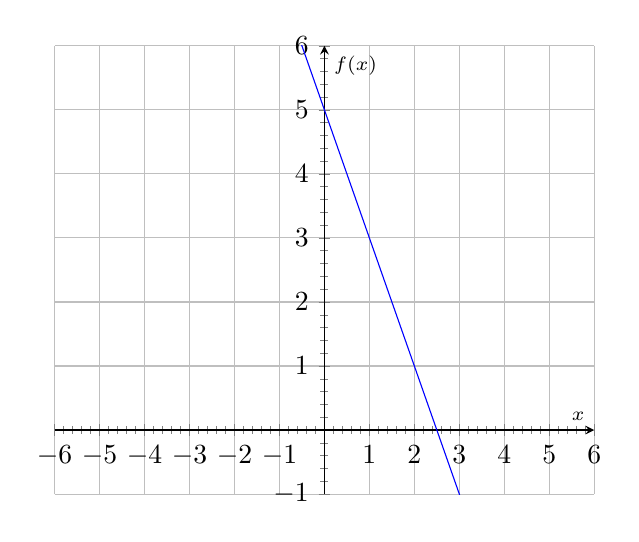
\begin{tikzpicture}[scale=1.0]
    \begin{axis}%
        [
            grid=major,
            xtick={-7,-6,...,7},
            minor x tick num=4, % 4 minor ticks => 5 subintervals
            xmin=-6,
            xmax=6,
            xlabel={\scriptsize $x$},
            axis x line=middle,
            ytick={-5,-4,...,6},
            minor y tick num=4,  % 4 minor ticks => 5 subintervals
            ymin=-1,
            ymax=6,
            ylabel={\scriptsize $f(x)$},
            axis y line=middle,
            no markers,
            samples=100,
            domain=-6:6,
        ]
        \addplot (x,{-2*x+5});
        \slopeTriangle{0.8}{0.1}{0.5}{1}{blue}; % USE OF MACRO.
    \end{axis}
\end{tikzpicture}